\documentclass[aspectratio=169]{beamer}
\hypersetup{pdfpagemode=FullScreen}
\usetheme[progressbar=frametitle]{metropolis}
\usepackage{appendixnumberbeamer}
\usepackage{listings}
\bibliographystyle{plainnat}
\usepackage{listings}
\usepackage{hyperref}
\usepackage{booktabs}
\usepackage{tikz}
\usepackage{tikzpeople}
\usepackage{biblatex}
\addbibresource{references.bib}
\usetikzlibrary{shapes,arrows}
\usepackage[scale=1]{ccicons}
% \usepackage{enumitem} % not compatible with enumerate in beamer class
\usepackage{xspace}
\newcommand{\themename}{\textbf{\textsc{metropolis}}\xspace}

\title{Competition}
% \subtitle{Subtítulo}
% \date{\today}
\date{May 30, 2022}
\author{Tensorboys}
\institute{Pattern Recognition}
% \titlegraphic{\hfill\includegraphics[height=1.5cm]{logo.pdf}}

\begin{document}

\maketitle

\begin{frame}{Agenda}
    \setbeamertemplate{section in toc}[sections numbered]
    \tableofcontents
\end{frame}
\section{Multi-layer Perceptron}
\begin{frame}[t]
    \frametitle{MLP}
    \begin{columns}
        \column{0.4\textwidth}
        \begin{itemize}
            \item We've tested multiple architecture from $784\times 2 \times 10$ to $784\times 512 \times 512\times 256 \times 128 \times 10$.
            \item This process was obviously automated.
            \item This yielded interesting results.
        \end{itemize}
        \column{0.6\textwidth}
        \begin{figure}[ht!]
            \centering
            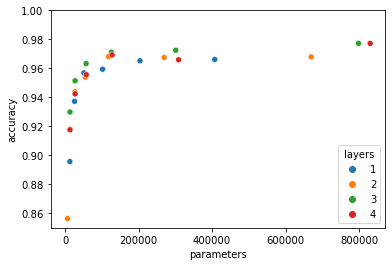
\includegraphics[width=0.6\textwidth]{figures/mlp_layers_global.png}
            \caption{Relation between parameters and accuracy for different model layers. We can see a rapid performance gain in the beginning, then not much difference for many more parameters }
            \label{fig:mlp}
        \end{figure}
    \end{columns}
\end{frame}

\begin{frame}[t]
    \frametitle{MLP}
    \begin{columns}
        \column{0.4\textwidth}

        \begin{itemize}
            \item 20 epochs and batch size of 128.
            \item Some good "light" architectures with 3-4 small layers
            \item For the competition: $784 \times 512 \times 128 \times 64 \times 10$ trained for 100 epochs
            \item Precision: 97.78\%
        \end{itemize}
        \column{0.6\textwidth}
        \begin{figure}[ht!]
            \centering
            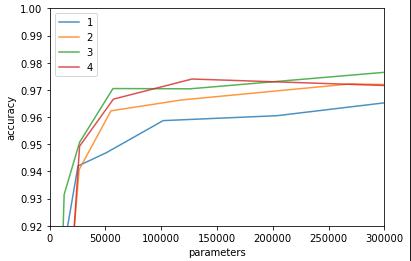
\includegraphics[width=0.6\textwidth]{figures/mlp_layers.png}
            \caption{Zoomed out version. Useful to find the best ratio between performance and size of model}
            \label{fig:mlp_zoomed}
        \end{figure}
    \end{columns}
\end{frame}
\section{Convolutional Neural Network}

\begin{frame}[t]
    \frametitle{CNN}
    \begin{columns}
        \column{0.3\textwidth}

        \begin{itemize}
            \item 20 epochs and batch size of 1024.
            \item Max Pooling after each convolution (could try without)
            \item one with bigger Kernel, one with a drop out layer after the flattening
            \item could go bigger but training time get annoying, keep things simple
        \end{itemize}
        \column{0.7\textwidth}
        \begin{figure}[ht!]
            \centering
            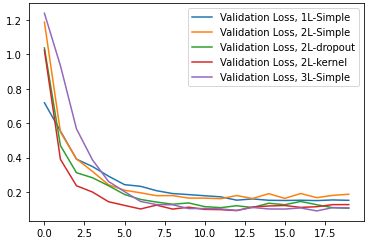
\includegraphics[width=0.7\textwidth]{figures/cnn_perf.png}
            \caption{Performance of the different model}
            \label{fig:cnn}
        \end{figure}
    \end{columns}
\end{frame}

\begin{frame}[t]
    \frametitle{CNN}

    

    \begin{columns}
        \column{0.3\textwidth}

        \begin{itemize}
            \item 50 epochs and batch size of 512.
            \item Trained on the whole training/test set available from before
            \item Precision: 99.34\%
        \end{itemize}
        \column{0.7\textwidth}
        \begin{figure}[ht!]
            \centering
            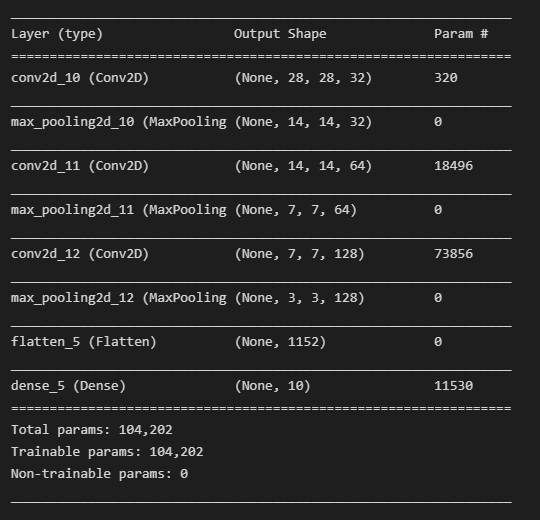
\includegraphics[width=0.7\textwidth]{figures/cnn_archi.png}
            \caption{Model used for the competition}
            \label{fig:cnn_model}
        \end{figure}
    \end{columns}
\end{frame}
\end{document}
